%%%%%%%%%%%%%%%%%%%%%%%%%%%%%%%%%%%%%%%%%
% Masters/Doctoral Thesis 
% LaTeX Template
% Version 2.5 (27/8/17)
%
% This template was downloaded from:
% http://www.LaTeXTemplates.com
%
% Version 2.x major modifications by:
% Vel (vel@latextemplates.com)
%
% This template is based on a template by:
% Steve Gunn (http://users.ecs.soton.ac.uk/srg/softwaretools/document/templates/)
% Sunil Patel (http://www.sunilpatel.co.uk/thesis-template/)
%
% Template license:
% CC BY-NC-SA 3.0 (http://creativecommons.org/licenses/by-nc-sa/3.0/)
%
%%%%%%%%%%%%%%%%%%%%%%%%%%%%%%%%%%%%%%%%%

%----------------------------------------------------------------------------------------
%	PACKAGES AND OTHER DOCUMENT CONFIGURATIONS
%----------------------------------------------------------------------------------------

\documentclass[
% The default document font size, options: 10pt, 11pt, 12pt
11pt, 
% Two side (alternating margins) for binding by default, uncomment to switch to one side
oneside,
% ngerman for German
english,
% Single line spacing, alternatives: singlespacing, onehalfspacing or doublespacing
onehalfspacing,
% Uncomment to enable draft mode (no pictures, no links, overfull hboxes indicated)
%draft,
% If the document is nolistspacing, onehalfspacing or doublespacing, uncomment this to set spacing in lists to single
onehalfspacing,
% Uncomment to add the list of figures/tables/etc to the table of contents
%liststotoc,
% Uncomment to add the main table of contents to the table of contents
%toctotoc,
% Uncomment to add space between paragraphs
parskip,
% Uncomment to not load the hyperref package
%nohyperref,
% Uncomment to get a line under the header
headsepline,
% Uncomment to place the chapter title next to the number on one line
chapterinoneline,
% Uncomment to change the layout of the declaration, abstract and acknowledgements pages to match the default layout
%consistentlayout,
% The class file specifying the document structure
]{MastersDoctoralThesis}

% Required for inputting international characters
\usepackage[utf8]{inputenc}

% Output font encoding for international characters
\usepackage[T1]{fontenc}
\usepackage{textcomp} % support the degree symbol

% Use the Palatino font by default
\usepackage{mathpazo}

% Use tu justify paragraphs
\usepackage{ragged2e}

% Use the bibtex backend with the authoryear citation style (which resembles APA)
\usepackage[backend=biber,natbib=true]{biblatex}
% MLA, APA, or IEEE? - https://www.overleaf.com/learn/latex/Biblatex_citation_styles
%\usepackage[style=apa, backend=biber]{biblatex}

% The filename of the bibliography
\addbibresource{mainBiblio.bib}

% Required to generate language-dependent quotes in the bibliography
\usepackage[autostyle=true]{csquotes}

% to set default colours
\usepackage{xcolor}
\definecolor{mygray}{gray}{0.5}

% for gantt charts
\usepackage{tikz}
\usepackage{gantt}

% to rotate pages in landscape
\usepackage{lscape}

% equation arrows with text
\usepackage{amsmath}

% insert degree celsius symbol
\usepackage{textcomp}

% include other pdf pages
\usepackage{pdfpages}

%----------------------------------------------------------------------------------------
%	MARGIN SETTINGS
%----------------------------------------------------------------------------------------

\geometry{
	paper=a4paper,      % Change to letterpaper for US letter
	inner=2.5cm,        % Inner margin
	outer=3.8cm,        % Outer margin
	bindingoffset=.5cm, % Binding offset
	top=1.5cm,          % Top margin
	bottom=1.5cm,       % Bottom margin
	%showframe,         % Uncomment to show how the type block is set on the page
}

%----------------------------------------------------------------------------------------
%	THESIS INFORMATION
%----------------------------------------------------------------------------------------

% Your thesis title, this is used in the title and abstract, print it elsewhere with \ttitle
\thesistitle{Fabrication of graphitic-carbon suspended nanowires through mechanoelectrospinning of photocrosslinkable polymers}

% Your supervisor's name, this is used in the title page, print it elsewhere with \supname and \cosupname
\supervisor{Dr. Héctor Alán \textsc{Aguirre} Soto}
\cosupervisor{Dra. Dora Iliana \textsc{Medina} Medina}

% Your examiner's name, this is not currently used anywhere in the template, print it elsewhere with \examname
\examiner{}

% Your degree name, this is used in the title page and abstract, print it elsewhere with \degreename
\degree{Master of Science in Nanotechnology (MNT)}

% Your name, this is used in the title page and abstract, print it elsewhere with \authorname
\author{Antonio Osamu \textsc{Katagiri} Tanaka}

% Your address, this is not currently used anywhere in the template, print it elsewhere with \addressname
\addresses{Estado de México, Atizapan de Zaragoza}

% Your subject area, this is not currently used anywhere in the template, print it elsewhere with \subjectname
\subject{Nanotechnology}

% Keywords for your thesis, this is not currently used anywhere in the template, print it elsewhere with \keywordnames
\keywords{nanotechnology, carbon, nano-wires, electrospinning, NFES}

% Your university's name and URL, this is used in the title page and abstract, print it elsewhere with \univname
\university{\href{https://tec.mx/}{Instituto Tecnonólogico y de Estudios Superiores de Monterrey}}

% Your university's campus name and URL, this is used in the title page and abstract, print it elsewhere with \campusname
\campus{\href{https://tec.mx/}{Campus Estado de México}}

% Your department's name and URL, this is used in the title page and abstract, print it elsewhere with \deptname
\department{\href{https://tec.mx/}{School of Engineering and Sciences}}

% Your research group's name and URL, this is used in the title page, print it elsewhere with \groupname
\group{\href{https://www.medinadora.com/people}{ITESM \campusname}}

% Your faculty's name and URL, this is used in the title page and abstract, print it elsewhere with \facname
\faculty{\href{https://samp.itesm.mx/Programas/VistaPrograma?clave=MNT16&modoVista=Default&idioma=ES&cols=0}{Faculty: Nanotechnology}}

\AtBeginDocument{
\hypersetup{pdftitle=\ttitle}          % Set the PDF's title to your title
\hypersetup{pdfauthor=\authorname}     % Set the PDF's author to your name
\hypersetup{pdfkeywords=\keywordnames} % Set the PDF's keywords to your keywords
}

\begin{document}

% Use roman page numbering style (i, ii, iii, iv...) for the pre-content pages
\frontmatter

% Default to the plain heading style until the thesis style is called for the body content
\pagestyle{plain} 

%----------------------------------------------------------------------------------------
%	TITLE/COVER PAGE
%----------------------------------------------------------------------------------------

\begin{titlepage}
\begin{center}

\vspace*{.06\textheight}
{\scshape\LARGE \univname\par} % University name

\begin{center}

\includegraphics[width=0.15\textwidth]{./Figures/uniLogo.png}
\end{center}

\vspace{0.5cm}
\textsc{\Large Masters Thesis Proposal}\\[0.5cm]      % Thesis type

\HRule \\%[0.5cm]                           % Horizontal line
{\huge \bfseries \ttitle\par}\vspace{0.0cm} % Thesis title
\HRule \\[0.5cm]                            % Horizontal line
 
\begin{minipage}[t]{0.4\textwidth}
\begin{flushleft} \large
\emph{Author:}\\

% Author name - remove the \href bracket to remove the link
\href{https://linkedin.com/in/osamu-katagiri-84b2b940/}{\authorname}
%\authorname
\end{flushleft}
\end{minipage}
\begin{minipage}[t]{0.4\textwidth}
\begin{flushright} \large
\emph{Principal Advisor:} \\
% Supervisor name - remove the \href bracket to remove the link
%\href{http://www.doramedina.com}{\supname}
\supname

\bigskip

\emph{Co-advisor and\\Director of Program:} \\
% Supervisor name - remove the \href bracket to remove the link
\href{https://www.medinadora.com/}{\cosupname}
%\cosupname
\end{flushright}
\end{minipage}\\[0.5cm]
 
\vfill

\large \textit{A thesis proposal submitted in fulfillment of the requirements\\ for the degree of
% University requirement text
\degreename}\\[0.25cm]
\textit{in}\\[0.25cm]
% Research group name and department name
\groupname\\\deptname\\[1cm]
 
\vfill

% Address and Date
{\addressname \text{, } \large \today}\\[4cm]
% University/department logo - uncomment to place it
%
\includegraphics{./Figures/uniLogo.png}
 
\vfill
\end{center}
\end{titlepage}

%----------------------------------------------------------------------------------------
%	COMMITTEE'S PAGE
%----------------------------------------------------------------------------------------

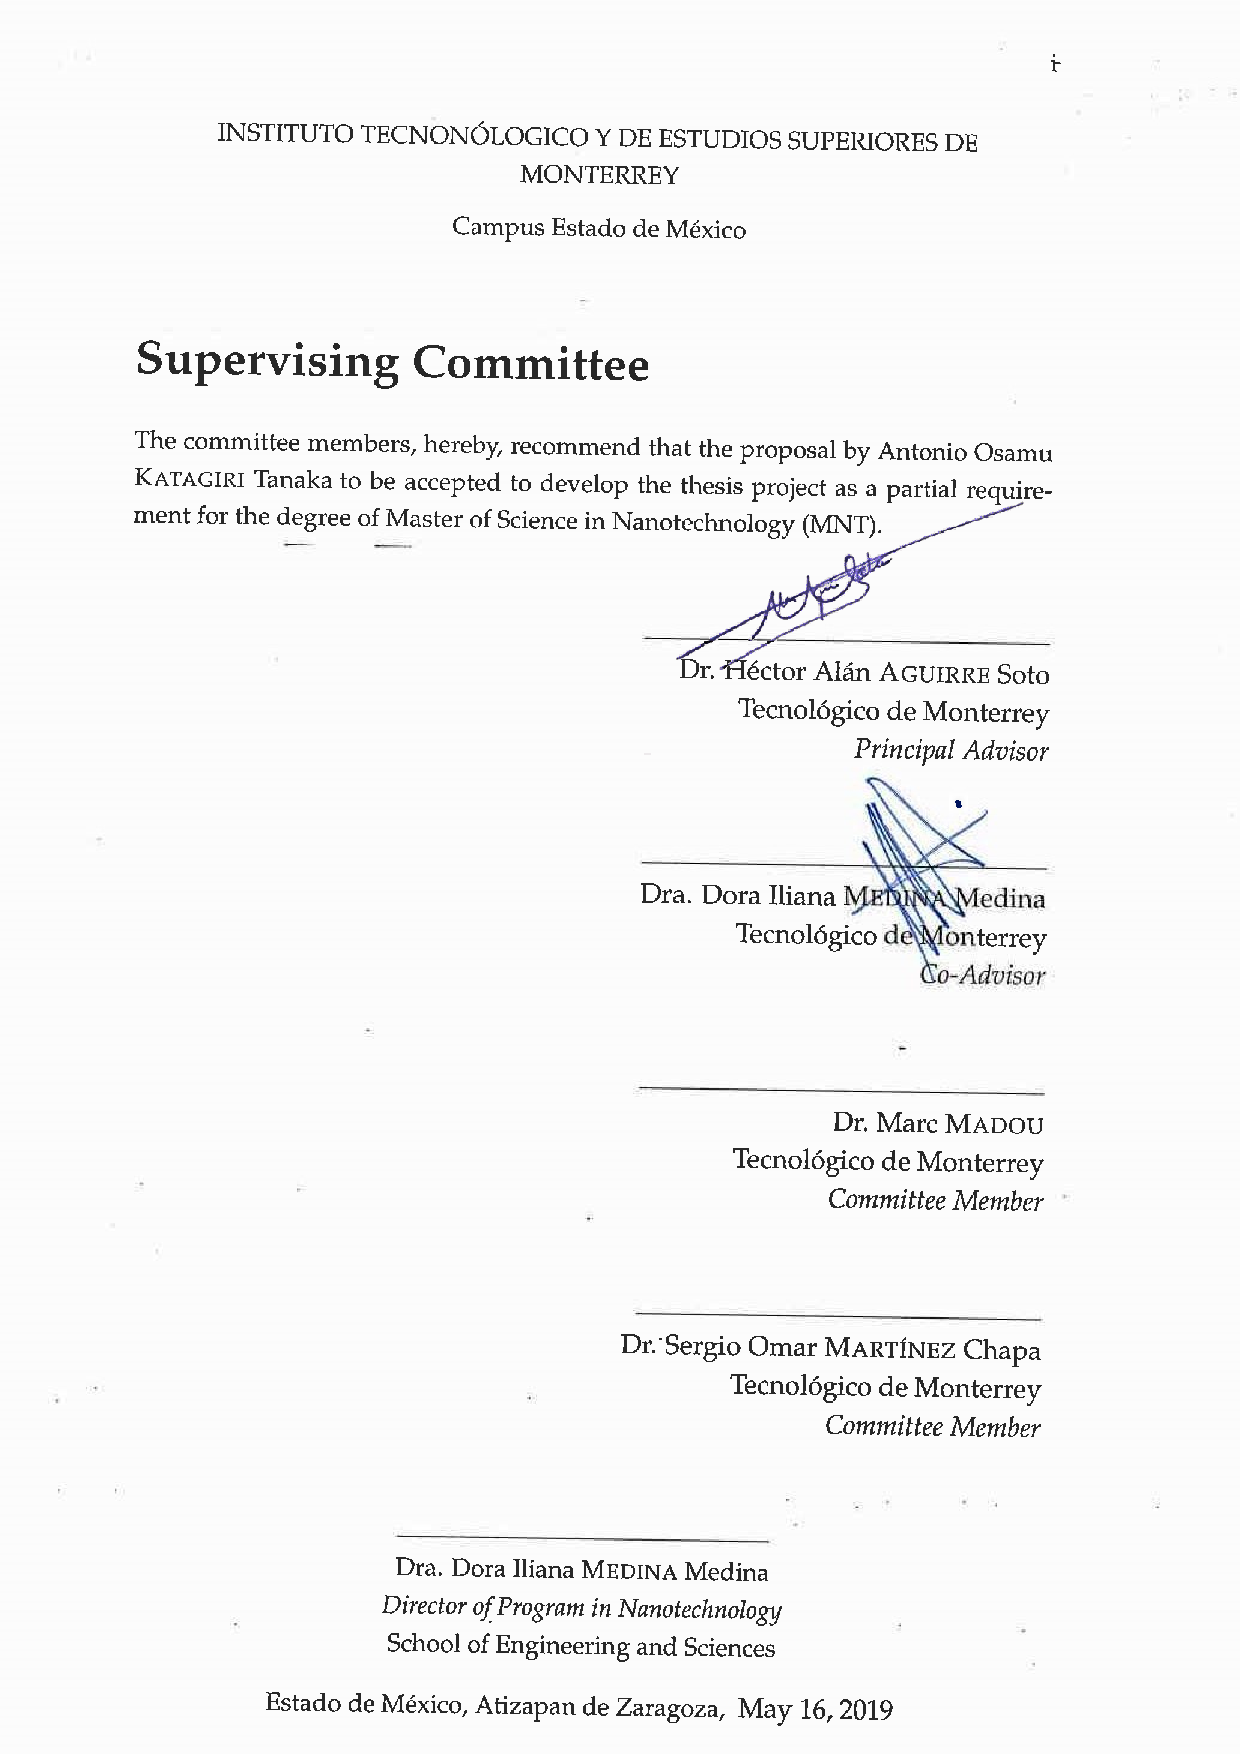
\includepdf[page=-]{./pdf/AlanDoraSigns}

%\begin{committee}
%\addchaptertocentry{\supervisingcommittee} % Add the the supervising committee to the table of contents
%The committee members, hereby, recommend that the proposal by \authorname \text{ }to be accepted to develop the thesis project as a partial requirement for the degree of \degreename.
%
%\begin{flushright} \large
%
%\bigskip
%\bigskip
%\medskip
%
%\noindent \rule[0.0em]{15em}{0.5pt}\\ % This prints a line for the signature
%%\href{http://www.alanaguirre.com}{\supname}
%\supname\\
%Tecnológico de Monterrey\\
%\emph{Principal Advisor}
%
%\bigskip
%\bigskip
%\medskip
%
%\noindent \rule[0.0em]{15em}{0.5pt}\\ % This prints a line for the signature
%%\href{http://www.alanaguirre.com}{\supname}
%\cosupname\\
%Tecnológico de Monterrey\\
%\emph{Co-Advisor}
%
%\bigskip
%\bigskip
%\medskip
%
%\noindent \rule[0.0em]{15em}{0.5pt}\\ % This prints a line for the signature
%%\href{http://www.alanaguirre.com}{\supname}
%Dr. Marc \textsc{Madou}\\
%Tecnológico de Monterrey\\
%\emph{Committee Member}
%
%\bigskip
%\bigskip
%\medskip
%
%\noindent \rule[0.0em]{15em}{0.5pt}\\ % This prints a line for the signature
%%\href{http://www.alanaguirre.com}{\supname}
%Dr. Sergio Omar \textsc{Martínez} Chapa\\
%Tecnológico de Monterrey\\
%\emph{Committee Member}
%
%\end{flushright}
%
%\vfill
%
%\begin{center}
%
%\bigskip
%\bigskip
%\medskip
%
%\noindent \rule[0.0em]{15em}{0.5pt}\\ % This prints a line for the signature
%\cosupname \\
%\emph{Director of Program in Nanotechnology}\\
%School of Engineering and Sciences\\
%%\href{http://www.doramedina.com}{\supname}
%
%\bigskip
%{\addressname \text{, } \large \today}\\[0cm]
%
%\end{center}
%\end{committee}
%
%\cleardoublepage

%----------------------------------------------------------------------------------------
%	LIST OF CONTENTS/FIGURES/TABLES PAGES
%----------------------------------------------------------------------------------------

\tableofcontents % Prints the main table of contents

\listoffigures % Prints the list of figures

%\listoftables % Prints the list of tables

%----------------------------------------------------------------------------------------
%	ABBREVIATIONS
%----------------------------------------------------------------------------------------

\begin{abbreviations}{ll} % Include a list of abbreviations (a table of two columns)

\textbf{CEM} & \textbf{C}ampus \textbf{E}stado de \textbf{M}éxico\\

\textbf{CNWs} & \textbf{C}arbon \textbf{N}ano-\textbf{w}ire\textbf{s}\\

\textbf{DC} & \textbf{D}irect \textbf{C}urrent\\

\textbf{EMS} & \textbf{E}lectro\textbf{m}echanical \textbf{S}pinning\\

\textbf{FFES} & \textbf{F}ar \textbf{F}ield de \textbf{E}lectro\textbf{s}pinning\\

\textbf{ITESM} & \textbf{I}nstituto \textbf{T}ecnonólogico y de \textbf{E}studios \textbf{S}uperiores de \textbf{M}onterrey\\

\textbf{MA} & \textbf{Ma}ssachusetts\\

\textbf{MEMS} & \textbf{M}icro\textbf{e}lectro\textbf{m}echanical \textbf{S}ystems\\

\textbf{MNT} & \textbf{M}aestría en \textbf{N}ano\textbf{t}ecnología \emph{(Master of Science in Nanotechnology)}\\

\textbf{MTY} & \textbf{M}on\textbf{t}erre\textbf{y} \emph{or} Campus \textbf{M}on\textbf{t}erre\textbf{y}\\

\textbf{NFES} & \textbf{N}ear \textbf{F}ield de \textbf{E}lectro\textbf{s}pinning\\

\textbf{USA} & \textbf{U}nited \textbf{S}tates of \textbf{A}merica\\

\textbf{UV} & \textbf{U}ltra\textbf{v}iolet\\

\end{abbreviations}

%----------------------------------------------------------------------------------------
%	ABSTRACT PAGE
%----------------------------------------------------------------------------------------

\begin{abstract}
\addchaptertocentry{\abstractname} % Add the abstract to the table of contents

Carbon nano-wires are versatile materials composed of carbon chains with a wide range of applications due to their high conductivity. Regardless of the high interest in the implementation of carbon nano-wires in several applications and devices, no feasible processes have been developed to fabricate carbon nano-wires with spatial control at a reasonable cost. Carbon nano-wires have been fabricated with the use of a photoresist, but little is known about polymers that can produce more conductive carbon nano-wires after pyrolysis. Various polymer solutions have been tested in near field electrospinning (NFES) and photopolymerization separately, however, few have been tested for nano-wire fabrication purposes through pyrolysis. The intention behind the thesis proposal is to implement rheology analyses of different polymer solutions to determine if they can be easily electrospun at low voltages and then fabricate nano-wires with them. This thesis work arises from the need to test a greater variety of polymers with the goal to design a polymer solution to fabricate carbon nano-wires with better conductivity than the current SU-8 polymeric nano-fibers. The research process will include the design of polymer solutions that can be electrospun, photopolymerized, and then pyrolyzed into conducting carbon nanowires. On the other hand, it is intended to engineer a newly designed polymer solution to achieve mass scale manufacturing of conductive carbon nano-wires in an inexpensive, continuous, simple and reproducible manner as central components for nano-sensors. \\

\noindent
\textbf{keywords:} \keywordnames
\end{abstract}

%----------------------------------------------------------------------------------------
%	PHYSICAL CONSTANTS/OTHER DEFINITIONS
%----------------------------------------------------------------------------------------

%\begin{constants}{lr@{${}={}$}l} % The list of physical constants is a three column table

% The \SI{}{} command is provided by the siunitx package, see its documentation for instructions on how to use it

%Speed of Light & $c_{0}$ & \SI{2.99792458e8}{\meter\per\second} (exact)\\
%Constant Name & $Symbol$ & $Constant Value$ with units\\

%\end{constants}

%----------------------------------------------------------------------------------------
%	SYMBOLS
%----------------------------------------------------------------------------------------

%\begin{symbols}{lll} % Include a list of Symbols (a three column table)

%$a$ & distance & \si{\meter} \\
%$P$ & power & \si{\watt} (\si{\joule\per\second}) \\
%Symbol & Name & Unit \\

%\addlinespace % Gap to separate the Roman symbols from the Greek

%$\omega$ & angular frequency & \si{\radian} \\

%\end{symbols}

%----------------------------------------------------------------------------------------
%	THESIS CONTENT - CHAPTERS
%----------------------------------------------------------------------------------------

\mainmatter % Begin numeric (1,2,3...) page numbering

\pagestyle{thesis} % Return the page headers back to the "thesis" style

% Include the chapters of the thesis as separate files from the Chapters folder
% Uncomment the lines as you write the chapters

\setlength{\parskip}{1.5em} % Paragraph spacing
%\RaggedRight
{\fontsize{12}{15} \selectfont

% Chapter Template

\chapter{Introduction} % Main chapter title

\label{Chapter:Introduction}

\subsubsection*{\color{mygray}[Chapter ready for review]}
% Introduction to the Context where the proposal is going to be carried out.
% Describe the Problematic Situation
% Briefly describe the problem, the relevant aspects and factors that are part of it.
% Justifify the relevance to provide a solution to the problem.
% Explain what has been previoulsy done to find a solution to the problem.
% Describe the proposed solution model
% State the expected achievements by solving this problema.
% Describe the organization of the document.

Carbon nano-materials are subjected to great interest for research purposes due to their various potential applications in diverse areas that take advantage of the nano-scale properties. \cite{Siddiqui2019} Carbon nano-materials are suitable for the catalysis, adsorption, carbon capture, energy and hydrogen storage, drug delivery, bio-sensing and cancer detection. \cite{Siddiqui2019} Some matchless properties that allow carbon nano-materials to be utilized within multiple functionalities include high porosity, distinguished structures, uniform morphologies, high stability, high magnetic properties and high conductivity. \cite{Siddiqui2019}

This document bestow a thesis proposal to perform a research to engineer and design a polymer solution to achieve mass scale manufacturing of high conductive carbon nano-wires with a reduced diameter in an inexpensive, continuous, simple and reproducible manner. The research intends to involve several manufacturing processes such as near field electrospinning, photopolymerization, pyrolization and carbonization, as they have shown to be promising methods for the fabrication of carbon nano-materials. \cite{Cardenas2017} See Figure \ref{fig:fabricationFlowChart}. A number of processes have been developed for specific purposes of polymeric nano-fibers, some include surface deposition, composites, and chemical adjustments. Polymeric nano-fibers must be also pyrolyzed to generate carbon nano-wires with conductive capabilities \cite{Madou2011} for electrochemical sensing and energy storage purposes.

\begin{figure}[th]
\centering
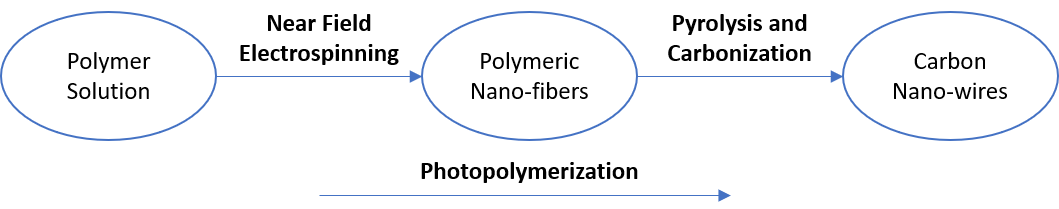
\includegraphics[width=0.95\textwidth]{./Figures/FabricationProcess.png}
\decoRule
\caption[Fabrication Process]{Fabrication process of carbon nano-wires to achieve through the proposed dissertation.}
\label{fig:fabricationFlowChart}
\end{figure}

Nanotechnology has explored different polymer patterning techniques to integrate carbon nano-wires structures. One technique is known as far-field electrospinning, a process in which electrified jets of polymer solution are dispensed to synthesize nano-fibers which then are pyrolyzed at high temperatures. One sub-technique derived from electrospinning is near field electromechanical spinning or EMS. EMS has proved to deliver high control in patterning polymeric nano-fibers. \cite{Cardenas2017}

The proposal is to continue the previous work done in regards of the synthesis of carbon nano-wires. Previous work includes the fabrication of suspended carbon nano-wires by two methods: electro-mechanical spinning and multiple-photon polymerization with a photoresist. \cite{Cardenas2017} This research proposal is intended to focus on electro-mechanical spinning processes only, to bring off polymer solutions that can be electrospun by near field electrospinning (NFES), photopolymerized and pyrolyzed into conducting carbon nano-wires. The polymer solutions described in \cite{Cardenas2017} are to be amended to achieve the goal mentioned in the previous statement.

Traditional near-field electrospinning or NFES allows large scale manufacturability combined with controlled guidance. \cite{Madou2011} However, the reported efforts required the use of electric fields in excess of 200 kV/m for continuous operation, resulting in limited control for nano-fiber patterning in traditional NFES processes. \cite{Madou2011} the current state-of-the-art synthesis processes for polymer nano-fibers lack to yield precise, inexpensive, fast, and continuous manufacturing properties.

%----------------------------------------------------------------------------------------
%	SECTION 1
%----------------------------------------------------------------------------------------



%-----------------------------------
%	SUBSECTION 1
%-----------------------------------



% Chapter Template

\chapter{Problem Definition and Motivation} % Main chapter title

\label{Chapter:ProblemDefinitionandMotivation}

% Describe the current situation of this problem.
Carbon nanowires have been fabricated with a photoresist by multiple-photon polymerization techniques. However little is known about polymers that can produce conductive carbon nanowires after pyrolysis.

% identifying the obstacles and the possible applications of your research.

% background of the problem (e.g. origins, previous attempts, etc.). 

% State the problem in detail mentioning all relative aspects, variables, relationships,

% stressing on the importance of finding a solution to the problem.



%----------------------------------------------------------------------------------------
%	SECTION 1
%----------------------------------------------------------------------------------------



%-----------------------------------
%	SUBSECTION 1
%-----------------------------------


% Chapter Template

\chapter{Hypothesis and Research Questions} % Main chapter title

\label{Chapter:HypothesisandResearchQuestions}

%\subsubsection*{\color{mygray}[Chapter ready for review]}
% The system/technique/parameter X is better, for task Y, than each of its rivals Z, in dimension W.

\section{Research Hypothesis}

The rheological properties of polymer solutions along with synthesis parameters (stage velocity, voltage, dispense rate) can be amended through rheological analyses to obtain a low voltage electrospun-able, photopolymerizable and graphitizable fibers for the synthesis of carbon nano-wires with specified dimensions (diameter and length).

\section{Research Questions}

\begin{itemize}
	\item{
	Is there any evidence of carbon nano-wire fabrication though electrospun-able and pyrozable polymer solutions?
	}
	\item{
	What are the process parameters to consider/control for the fabrication processes of carbon nano-wires? 
	}
	\item{
	What rheological properties are to be controlled/tested to deliver a electrospun-able and pyrozable polymer solution?	
	}
	\item{
	Are there any efforts employed to the design of polymer solutions that can be electrospun, photopolymerized, and pyrolyzed into conducting carbon nanowires?
	}
	\item{
	Are the optimal fabrication parameters defined \cite{Cardenas2017} for the synthesis of carbon nano-wires through near-field electromechanical spinning?	
	}
\end{itemize}

%----------------------------------------------------------------------------------------
%	SECTION 1
%----------------------------------------------------------------------------------------



%-----------------------------------
%	SUBSECTION 1
%-----------------------------------


% Chapter Template

\chapter{Objectives} % Main chapter title

\label{Chapter:Objectives}

%----------------------------------------------------------------------------------------
%	SECTION 1
%----------------------------------------------------------------------------------------



%-----------------------------------
%	SUBSECTION 1
%-----------------------------------


In view of the manufacturing and surface chemistry challenges posed by CNW biosensor
fabrication, the following dissertation is divided in two central objectives:

1) To explore the feasibility of using advanced additive manufacturing techniques to improve the reproducibility of CNW production in the nanoscale range.20 In particular, EMS and Direct Femtosecond Laser Writing (DLW) techniques will be studied and tested in terms of their fabrication parameters. Furthermore, morphological and electrical characterization of the obtained samples will be key in the discussion and assessment of this objective.

2) To study the surface chemistry of CNWs as a material for biomolecule immobilization. The goal will be to explore a functionalization technique that will allow the surface modification of GC to achieve the immobilization of a biomolecule. GC will be studied in particular since it is the predominant material obtained from advanced manufacturing techniques like EMS46 and TPP.50
% Chapter Template

\chapter{Related Work} % Main chapter title

\label{Chapter:RelatedWork}

%\subsubsection*{\color{mygray}[Chapter under work]}

%----------------------------------------------------------------------------------------
%	SECTION 1
%----------------------------------------------------------------------------------------

\section{Role of rheological properties in near field electrospun fibers morphology \cite{Flores2017}}

Flores studied SU-8 2002 polymer solutions in cyclopentanone with poly(ethylene) oxide (PEO) and tetrabutylammonium tetrafluoroborate (TBATFB). For that purpose, several samples were prepared with the adequate amounts of PEO and TBATFB with 5 $m l$ of SU-8 2002 and stirred at 160 $r p m$ for one hour at 75 $^\circ C$ in the absence of light. A 5 $m l$ syringe was used to extract the solution from the preparation vial. Finally the syringe was placed upside down for 24 hours to get rid of any bubbles within the solution. Table \ref{tbl:FloresSamples} lists the set of samples that were prepared as values in $w t \%$, dissolved in SU-8 2002.

\begin{table}[th]
\caption{Set of prepared samples}
\begin{center}
\begin{tabular}{ c c c c c c c } 
\hline
\text{} & \multicolumn{2}{c}{Serie A} & \multicolumn{2}{c}{Serie B} & \multicolumn{2}{c}{Serie C} \\
\hline
Sample & PEO & TBATFB & PEO & TBATFB & PEO & TBATFB \\
\hline
1 & 0.00 & 0.00 & 0.00 & 0.50 & 0.50 & 0.00 \\
2 & 0.25 & 0.25 & 0.25 & 0.50 & 0.50 & 0.25 \\
3 & 0.50 & 0.50 & 0.50 & 0.50 & 0.50 & 0.50 \\
4 & 0.75 & 0.75 & 0.75 & 0.50 & 0.50 & 0.75 \\
5 & 1.00 & 1.00 & 1.00 & 0.50 & 0.50 & 1.00 \\
\hline
\label{tbl:FloresSamples}
\end{tabular}
\end{center}
\end{table}

All the samples were executed in a rheometer (Physica MCR 301, Anton Paar) with a cone-and-plane geometry of diameter 24.979 $m m$, angle 4.014$^\circ$ and truncation of 249 $\mu m$. The measurements were performed at a temperature of 25 $\pm$ 0.1 $^\circ C$. For amplitude sweep measurements, the angular frequency was settled at 10 $s^{-1}$, and the percentage amplitude gamma $\% \gamma$, was varied from 0.1 to 1000\%. In flow curve tests, shear rate was applied from 0.1 to 100 $s^{-1}$. For frequency sweeps, the percentage of amplitude gamma, $\% \gamma$, was varied from 0.1 to 100 $s^{-1}$. During the measurements, the rheometer sample area was saturated with cyclopentanone to avoid solvent evaporation.

\subsection{Rheological Characterization : \textbf{Amplitude Sweep}}
The "Serie A`` result measurements indicate that the storage modulus $G'$ is smaller than the loss modulus $G''$. Both moduli have a parabolic behaviour. At low deformation the values of the moduli increase until they become stable at between 1 and 10 $\% \gamma$. After the stabilization, both modulus start to decrease. The increase of PEO and TBATFB concentration $G'$ and $G''$ also increase. Figure \ref{fig:SerieAampSweep} shows the amplitude sweep for the samples of "Serie A``.

\begin{figure}[th]
\centering
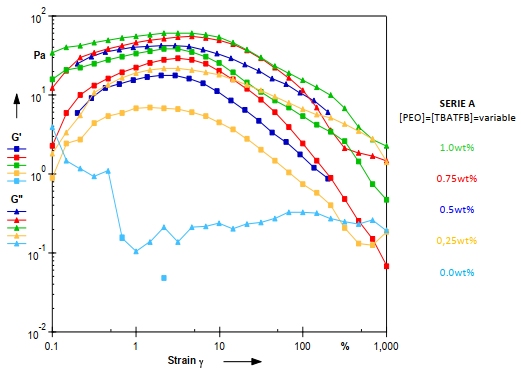
\includegraphics[width=0.75\textwidth]{./Figures/SerieAampSweep.png}
\decoRule
\caption[Serie A - Amplitude Sweep]{Serie A - Amplitude Sweep}
\label{fig:SerieAampSweep}
\end{figure}

The results within Figure \ref{fig:SerieAampSweep} showed that no clear linear viscoelastic region is present. The material has influenced by small deformations, hence it is very sensible to external forces. No yield point was encountered as the moduli separate from each other with the increase of deformation.

Figure \ref{fig:SerieBampSweep} illustrates the results obtained from the amplitude sweeps of Serie B samples. As shown in the figure, the concentration of 0 $w t \%$ shows a constant viscous modulus at 0.2 $Pa$. the 0.25 $w t \%$ concentration sample presented a similar behaviour to the 0 $w t \%$ sample but with a constant value of $G'$ at 2 $Pa$. The other concentrations show a similar parabolic behaviour as the ones in Serie A.

\begin{figure}[th]
\centering
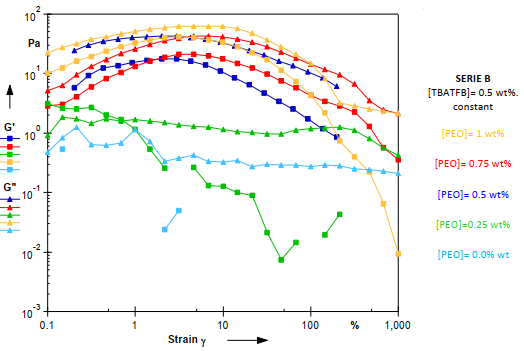
\includegraphics[width=0.75\textwidth]{./Figures/SerieBampSweep.png}
\decoRule
\caption[Serie B - Amplitude Sweep]{Serie B - Amplitude Sweep}
\label{fig:SerieBampSweep}
\end{figure}

\begin{figure}[th]
\centering
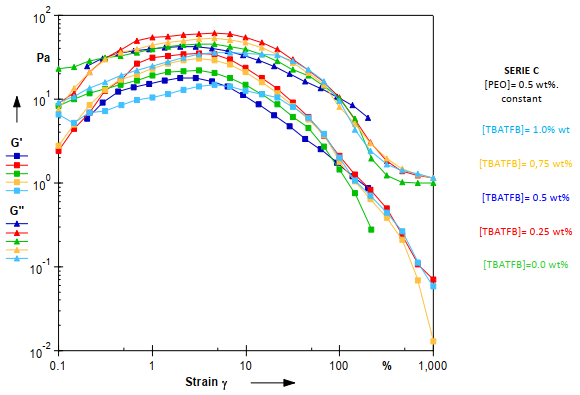
\includegraphics[width=0.75\textwidth]{./Figures/SerieCampSweep.png}
\decoRule
\caption[Serie C - Amplitude Sweep]{Serie C - Amplitude Sweep}
\label{fig:SerieCampSweep}
\end{figure}

The amplitude sweep results of Serie C are depicted in Figure \ref{fig:SerieCampSweep}. Similar to series A and B, results show that the storage modulus $G'$ is smaller than the loss modulus $G''$ with a parabolic behaviour. Typically, the amplitude sweep is to determine the amplitude to be used in frequency sweeps. The amplitude determined by the amplitude sweeps shall keep the material structure undisturbed is known as the linear viscoelastic region (LVER). However, no LVER was found in the samples. For that reason, the percentage of amplitude gamma $\% \gamma$ was found by trial and error. Flores discovered that a $\% \gamma = 20$ has the best performance. 

\subsection{Rheological Characterization : \textbf{Flow Curve}}
Figure \ref{fig:SerieAflowCurve} shows evidence that the equal increase of PEO and TBATFB concentrations result in an increase of shear viscosity rate $\gamma$. for concentrations from 1.00 to 0.25 $w t \%$, a slight increase of flow curve strain $\eta$ for low shear rates to 0.3 $s^{-1}$. For shear rates greater than 0.3 $s^{-1}$, the $\eta$ starts to decrease, as the polymer entanglements start to break apart, reducing friction between the polymer threads and therefore the viscosity also is reduced. The solution samples show a Newtonian-like behaviour and that may be caused by the use of the solvent cyclopentanone and by the small sized SU-8 2002 molecules.

\begin{figure}[th]
\centering
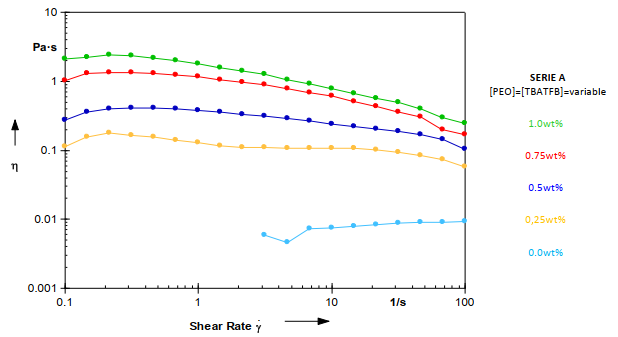
\includegraphics[width=0.75\textwidth]{./Figures/SerieAflowCurve.png}
\decoRule
\caption[Serie A - Flow curve]{Serie A - Flow curve}
\label{fig:SerieAflowCurve}
\end{figure}

From the results in Figure \ref{fig:SerieAflowCurve}, it is noticeable that the addition of small amounts of PEO and TBATFB cause a change of one order of magnitude in shear viscosity in small concentration and a triple change in high concentrations.

Series B flow curve results (Figure \ref{fig:SerieBflowCurve}) do not show a clear correlation between PEO concentrations and shear viscosity. For PEO of 1 $w t \%$, a slow increase in $\eta$ is present with the increase of shear rate, after $\gamma$ drops from 2 to 0.8 $Pa s$, a shear thinning behaviour is present. For 0.50 and 0.75 $w t \%$ concentrations, a shear thinning behaviour is present throughout the plot. For the 0.50 $w t \%$ sample, viscosity value varied between 0.2 and 0.4 $Pa s$; and between 0.5 and 2.0 $Pa s$ for the 0.75 $w t \%$ sample. Viscosity is stabilized at 0.1 $Pa s$ when the shear rate is between 1 and 20 \% for the sample of PEO $w t \%$. After stabilization, the viscosity decreases from 0.1 to 0.02 $Pa s$ for shear rates between 20 to 100 $s^{-1}$. For PEO 0.00 $w t \%$, a high variation is present in viscosity readings due to the presence of electrolytes cause amendments in the polymer chain within the solution.

\begin{figure}[th]
\centering
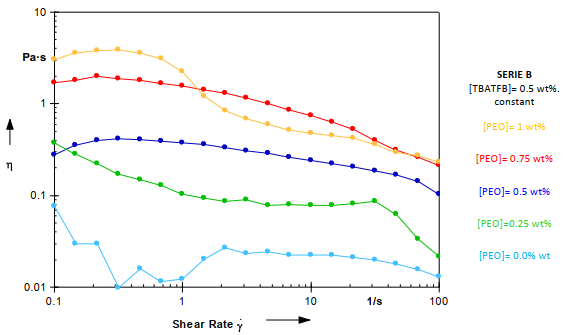
\includegraphics[width=0.75\textwidth]{./Figures/SerieBflowCurve.png}
\decoRule
\caption[Serie B - Flow curve]{Serie B - Flow curve}
\label{fig:SerieBflowCurve}
\end{figure}

The flow curve results of Serie C are presented in Figure \ref{fig:SerieCflowCurve}. The sample with 1 $w t \%$ TBATFB concentration shows a shear thinning behaviour for shear rates varying between 0.1 to 15 $s^{-1}$. The 1 $w t \%$ sample describes a drop in viscosity for shear rates between 15 to 20 $s^{-1}$ followed by a stable state. A similar behaviour is observed for concentration of 0.75 $w t \%$. and less evident for 0.0 $w t \%$. For concentrations of 0.5 $w t \%$ and 0.25 $w t \%$ the behaviour of the shear viscosity is similar.

\begin{figure}[th]
\centering
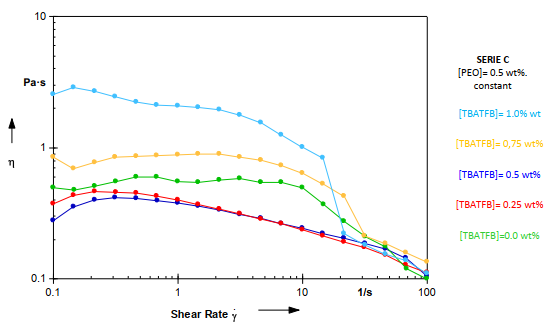
\includegraphics[width=0.75\textwidth]{./Figures/SerieCflowCurve.png}
\decoRule
\caption[Serie C - Flow curve]{Serie C - Flow curve}
\label{fig:SerieCflowCurve}
\end{figure}

\subsection{Rheological Characterization : \textbf{Frequency Sweep}}
Figure \ref{fig:SerieAfreqSweep} shows that the solution with the lowest concentration of PEO and TBATFB has a decreasing behaviour of the viscosity, but for values greater to 3 $s^{-1}$ in frequency, the viscosity starts to increase. The solutions from 0.25 $w t \%$ to 1.00 $w t \%$ have the same shear-thinning behaviour. A direct relation between the concentrations and the viscosity values is discovered, where a small drop of viscosity is presented with the decrease of additive concentration.

\begin{figure}[th]
\centering
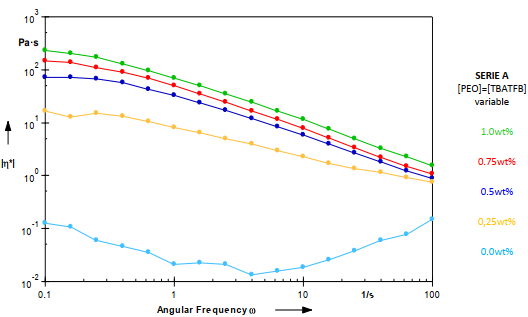
\includegraphics[width=0.75\textwidth]{./Figures/SerieAfreqSweep.png}
\decoRule
\caption[Serie A - Frequency Sweep]{Serie A - Frequency Sweep}
\label{fig:SerieAfreqSweep}
\end{figure}

Figure \ref{fig:SerieBfreqSweep} shows the frequency sweep results from Serie B. The presented behaviour is similar to Serie A. for the lower concentrations of PEO, the equipment has not enough sensibility to make measurements of the storage modulus because this one is very low. At PEO 0.25 $w t \%$, the viscosity remains almost constant at 1 $Pa s$, but as in Serie A a little variation of viscosity is presented at the lowest values of angular frequency. On the other hand, for the 0.5, 0.75 and 1.00 $w t \%$ concentrations, the viscosity is similar. At 100 $s^{-1}$, the three high concentration samples converge to 2 $Pa s$. It is imperative to assume that 0.5 $w t \%$ is the critical concentration, under this concentration the systems presents different behaviours since the molecules have enough room to diffuse and break entanglements. When the critical entanglement concentration is exceeded, the polymer threads overlap and become tangled, therefore no more entanglements are no longer possible.

\begin{figure}[th]
\centering
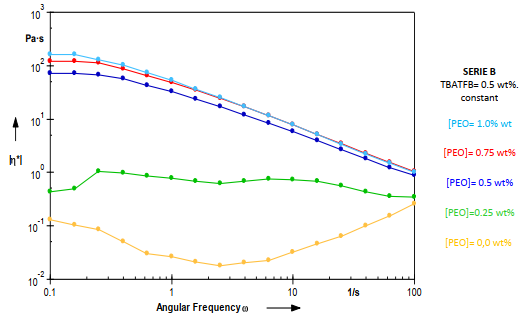
\includegraphics[width=0.75\textwidth]{./Figures/SerieBfreqSweep.png}
\decoRule
\caption[Serie B - Frequency Sweep]{Serie B - Frequency Sweep}
\label{fig:SerieBfreqSweep}
\end{figure}

The frequency sweep behaviours of Serie C are presented in Figure \ref{fig:SerieCfreqSweep}. The figure does not indicate a clear correlation between the viscosity and the addition of TBATFB. All samples have a similar behaviour and magnitude, except for the 0.75 $w t \%$ TBATFB concentration sample as it presents a non uniform behaviour. At low frequencies, the viscosity increases, then it remains constant at 20 $Pa s$ until a frequency value of 4 $s^{-1}$; the viscosity drastically decreases to 1 $Pa s$ and remains constant at that value. The 1.00 $w t \%$ sample has a decreasing viscosity behaviour at higher angular frequencies. 

\begin{figure}[th]
\centering
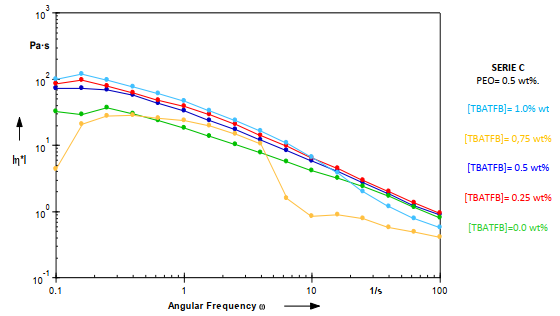
\includegraphics[width=0.75\textwidth]{./Figures/SerieCfreqSweep.png}
\decoRule
\caption[Serie C - Frequency Sweep]{Serie C - Frequency Sweep}
\label{fig:SerieCfreqSweep}
\end{figure}

Flores work \cite{Flores2017} carried out a series of experiments in order to correlate the rheological properties of polymer solutions used in electro-mechanical spinning processes for the fabrication of carbon micro structures. Shear flow and dynamic measurements tests such as flow curves, amplitude sweeps and frequency sweeps were carried in an oscillatory rheometer to study the rheological behaviour of polymeric solutions of SU-8 2002, an epoxy-based negative photoresist, Poly(ethylene) oxide (PEO), a flexible, non-ionic polymer, and TBATFB (Tetrabutylammonium tetrafluoroborate) that acts as an electrolyte.

The concentrations of additives were varied from 0 $w t \%$ to 1.0 $w t \%$ with increments of 0.25. To observe the effects of each additive it was proposed a set of concentrations where both additives were equally varied (Serie A), TBATFB was constant the only PEO variations (Serie B), and PEO constant concentration with TBATFB variations (Serie C). It was found that the variation of the additives (PEO and TBATFB) affects the
rheological behavior of the solution. Typically, the addition of PEO increase the
elongational and shear viscosities while the addition of TBATFB modifies this property
but in a non-predictable manner. The solutions do not present yield stress as can be
seen in Amplitude Sweep and Frequency Sweep measurements.

\clearpage

\section{Advanced Manufacturing Techniques for the Fabrication and Surface Modification of Carbon Nanowires \cite{Cardenas2017}}

As stated by Cardenas \cite{Cardenas2017}, the following parameters play an important role in the graphitic content on the fabrication of carbon nano-wires through electrospinning:

\begin{enumerate}
\item The thickness of the produced polymeric wires,
\item the chemical composition and viscoelasticity of the polymeric solution,
\item the molecular alignment of the polymer,
\item the heat treatment temperature,
\item the mechanical pulling on the polymer jet during electrospinning,
\item the alifnment of polymer chains induced by the presence of an electric field, and
\item the catalysts and solvents within the polymer solution.
\end{enumerate}

Cardenas reviewed different polymer fabrication techniques and materials to produce carbon nano-wires. Within Cardenas' work the following parameters were evaluated to study the desirable characteristics for building highly sensitive sensor devices: a) the chemical composition and viscoelasticity of the polymer solution, b) the thickness of the produced polymeric wires, c) the mechanical pulling on the polymeric jet during electrospinning, and d) the alignment of the polymer chains induced by the presence of an electric field. Cardenas' work states that various methods are implemented to produce nanofibers, such as laser ablation, chemical vapor deposition, discharge, and vapour growth. However, those techniques are abandoned due to their low yield output and expensive equipment. Whereas electrospinning (ES) of polymer solutions is a promising technique for simple and inexpensive fabrication of carbon nano-wires, which can be combined with a moving collector to yield even thinner fibers.

The production of carbon sstructures involves to main procedures: a) polymer patterning such as photolithography, electrospinning, Computer Numerical Control (CNC), moulding, hot embossing, and recently, Multiple Photon Polymerization; and b) carbonization, which induces further thinning of the patterned polymer and its conversion into carbon. Cardenas conducted some experiments to characterize and analyse carbon nano-wires. Polymeric SU-8 nano fibers were produced by two different methods; for each method different polymer solutions were employed.

\subsection{Method 1 : }

\subsubsection{Polymer Solution}
The polymeric solution was composed by 2 $ml$ of SU-8 2002 mixed with 0.5 $w t \%$ of PEO and 0.5 $w t \%$ of TBATFB to increase its conductivity and yield soother polymer jets during electrospinning. Magnetic stirring was performed for 1 $hr$ at 75 \textdegree{}$C$ with $rpm$ values between 100 and 150.

\subsubsection{Deposition}
A voltage around 100 $V$ was applied between a dispensing needle and the collector stage. The needle to collector distance was set to 100 $\mu m$. The collector was attached to a mechanically motorized stage, which allowed the SU-8 nanofibers patterning into the SU-8 microstructures. Three different stage velocities were tested (20,40 and 60 $mm/s$) to study the influence on the wire geometry. Acceleration of the stage was set to 500 $mm/s^{2}$. After deposition, samples were exposed to UV light for 45 $min$ to complete cross-linking.

\subsection{Method 2 : }

\subsubsection{Polymer Solution}
The solution was composed of 4 $ml$ of SU-8 2025, 4 $mg$ of TBATFB and 80 $\mu L$ of SU-8 thinner. The solution was stirred for 1.5 $hrs$ at 100 $rpm$ at 75 \textdegree{}$C$.

\subsubsection{Deposition}
To pattern the fiber exactly on top of the SU-8 electrodes, a routine was set to move the needle relative to the collector. The polymer solution was dispensed at a rate of 8.847 $nL / min$ using a programmable syringe pump. A voltage of 200 $V$ was applied between the collector plate and the needle tip, and the polymer solution was allowed to flow for between 15 to 30 $min$ until it was stable. A higher voltage had to be applied compared to Method 1 due to the higher viscosity of the SU-8 2025 solution. Once a steady flow was achieved, the collector was moved relative to the needle tip using the motorized stage. The mechanical parameters used during were: a) velocity of 5000 $\mu m/s$, an acceleration of 2500 $\mu m/s^{2}$. The sample was exposed to UV light for 45 min to ensure complete cross-linking of the deposited SU-8 nanofiber.

\subsection{Results and Discussion}
To test the possibility of using SU-8 to fabricate carbon nano-wires, samples were pyrolyzed in an inert environment. Samples prepared by Method 1 failed the pyrolyzation as the deposited wires were mostly liquid before carbonization. The fibers produced by Method 2 had a yeild rate of 81 $\%$. The diameters after pyrolysis were analyzed and measured using SEM micrographs.

Cardenas \cite{Cardenas2017} states that the geometry of the carbon nano-wires is also an important characteristic that affects the carbon structure conductivity, mechanical and thermal characteristics and crystallinity. The conducted experiments showed some techniques and materials that have been applied to fabricate carbon nano-wires, as well as the effects that fabrication parameters have on the final geometry of the carbon structures. The newly technique of electro-mechano-spinning (EMS) involved new polymer solutions along with a systematic deposition process. Cardenas found that the EMS proposed manufacturing technique yielded normally distributed diameters of 204 $nm$ with low variability, which is significantly reduced the uncertainty in the fabrication of carbon nano-wires.

\section{Effect of pyrolysis process parameters on electrical, physical, chemical and electro-chemical properties of SU-8-derived carbon structures fabricated using the C-MEMS process \cite{Pramanick2018}}


%-----------------------------------
%	SUBSECTION 1
%-----------------------------------



% Chapter Template

\chapter{Theoretical Framework} % Main chapter title

\label{Chapter:TheoreticalFramework}

%\subsubsection*{\color{mygray}[Chapter under work]}
% Background and state-of-the-art
% This involves a thorough state-ofthe-art bibliographic review, the building of a formal foundation, the study of related techniques, analysis and awareness of previous works and study of fundamental aspects that can help carry on your research.

\section{Photoresists}
The electronic industry requires a sustainable raw material supply for its development \cite{Sutikno2016}. Photoresists are a type of raw material used in microelectronics, which is composed by four main elements: a polymer (resin), a photoactive compound, a solvent, and an additive \cite{Schuster2009}. The additive requires to be with low molecular weight as it is intended to act as a photosensitive material. Photoresists are used within the manufacturing process of printed circuit boards \cite{Staab2011}. Photoresists are classified into two categories. The resist is defined as positive if the radiation exposed material is soluble in photoresist developer; otherwise, for negative photoresist the exposed material remains to stay in the photoresist surface as it crosslinks upon exposure \cite{Landis2011,Sharma2012}. In the manufacturing process of a semiconductor, the radiation sources which are often used in a lithography process are ultraviolet (UV) and X-ray \cite{Mekaru2015}.

The polymeric material is available on the broad market either in liquid or solid state; \emph{MicroChem Corp.} (Westborough, MA, USA) is the principal provider of SU-8 photoresist. SU-8 and similar photoresists are inexpensive with good adhesion on the semiconductor surface and high sensitivity \cite{Staab2011}. Epoxy resins are copolymer-thermosetting plastics which are normally produced by a chemical reaction process that involves epichlorohydrin and bisphenol-A compound \cite{Singla2010}. An epoxy-based polymer is typically used to produce patterns by lithography with the application of UV radiation. Lithography is a technique to transfer patterns from a mask and then transferred onto the substrate \cite{Landis2011,Xu2014}. SU-8 is a epoxy-based negative photoresist with the advantages of being inexpensive with good mechanical properties, good chemical resistance, and good electrical isolation \cite{Xu2014}. SU-8 photoresists are used in the production processes of MEMS \cite{Zhang2001}. Photoresist-wise, the contrast and quality level of UV radiation lithography is affected by the wavelengths of radiation sources. The higher the sensitivity of the material, the better is the lithography process as it absorbs radiation energy with ease to perform photochemical reactions in forming patterns \cite{Zhang2001}.

In summary, a photoresist is an "epoxy-based resin (polymeric) material which changes its dissolution rate in a liquid solvent, called a developer, under high energy radiation.`` \cite{Landis2011}

\section{Electro-Mechanical Spinning}
Diverse polymer patterning techniques have been developed for the fabrication of nano-fibers, such as arc discharge \cite{Wang2007}, chemical vapor deposition, laser ablation \cite{Ren1998}, and vapor growth \cite{Nadarajah2008}. Nonetheless, those processes are expensive due to either the low product yield or the expensive equipment required. The electrospinning method (invented by Formhals Anton in 1934) can produce fibers with a range of diameters between 10 $n m$ and 10 $\mu m$ \cite{Jayaraman2003,Anton1930} from a polymer solution under the influence of an electrostatic force. The applied electric field and solution conductivity and viscosity is an important parameter the affects the fiber diameter during the spinning along with other parameters such as jet length, solution viscosity surrounding gas, flow rate and the collector geometry \cite{Anton1938,Larrondo1981,Baumgarten1971,Shin2001}.

Even though electrospinning is an old invention \cite{Anton1930}, it is currently a trending topic among researchers \cite{Huang2003,Reneker2008,Schiffman2008}. One of the reasons electrospinning is to be studied is its potential to fabricate polymer nano-fibers from a variety of polymers. The technique allows the production of thin continuous fibers with ease, with diameters down to 3 $n m$ in some cases, which is something difficult to achieve by other techniques. Furthermore, the basic set-up can be modified with ease to fabricate different fibers with diversified functionalities with different materials. The produced fibers can be aligned or unaligned. Besides, the electrospinning equipment is inexpensive and of small size, compared to the equipment of standard spinning techniques. On the other hand, the understanding of the electrospinning process has improved in the last years \cite{Li2012}. As Reneker and Yarin state: "Electrospinning has rapidly changed fiber making from a capital intensive, large scale process to a low cost, broadly applicable method that manufactures fibers on a laboratory bench, to serve diverse needs ranging from materials science and technology to life sciences and clinical medicine.`` \cite{Reneker2008}

The main components of the electrospinning technique are the fluid control unit (e.g. syringe pump) and a DC power supply. The process also requires a target electrode or combination of electrodes on which the fibers can be collected. Figure \ref{fig:FFES} describes a typical electrospinning set-up. \cite{Li2012}

\begin{figure}[th]
\centering
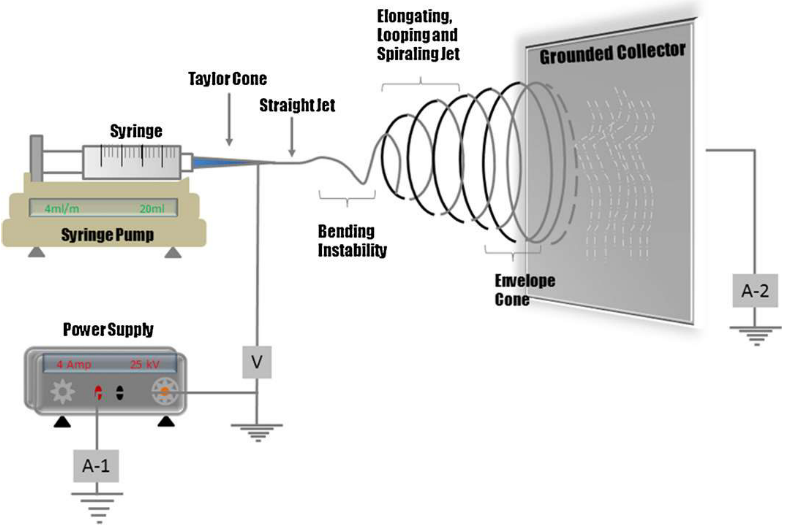
\includegraphics[width=0.75\textwidth]{./Figures/FFES.png}
\decoRule
\caption[Far Field Electrospinning set-up]{Typical far field electrospinning (FFES) set-up \cite{Li2012}.}
\label{fig:FFES}
\end{figure}

Two sub-techniques can be derived from electrospinning depending on the distance between the dispensing electrode and the collector. The process in which the electrospun jet can be controlled near the tip is called NFES or near-field electrospinning. \cite{Cisquella-Serra2019} Moreover, if the distance between the collector and the dispensing needle is greater, the configuration is known as FFES or far-field electrospinning. \cite{Nataraj2012} The difference between NFES and mechano-electrospinning is the presence of a mechanical collector that allows higher precision when patterning. Figure \ref{fig:NFES} shows a typical near field mechano-electrospinning apparatus.

\begin{figure}[th]
\centering
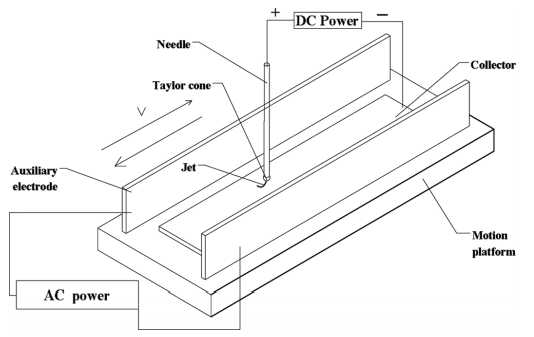
\includegraphics[width=0.75\textwidth]{./Figures/NFES.png}
\decoRule
\caption[Near Field Electrospinning set-up]{Typical near field electrospinning (NFES) set-up \cite{Zhu2016}.}
\label{fig:NFES}
\end{figure}

\section{Pyrolysis} \label{sec:pyrolysis}
Pyrolysis is a technique that involves heating of biomass in the absence of air or oxygen at a maximum pyrolysis temperature. A small amount of oxygen can burn the structures and make them unusable \cite{Pramanick2018}. Once the maximum pyrolysis temperature is reached, the temperature remains constant to produce solid char, liquids, and non-condensable products. In most cases the liquid product is the main interest of the pyrolysis process, and the properties of the pyrolysis products depend on the maximum pyrolysis temperature and the heating rate \cite{Pramanick2018,Basu2018}.

The heating of large biomass molecules results in decomposition. The pyrolysis decomposition process comprises char, liquids (condensable gases) and non-condensable gases; where the condensable gases may suffer further decomposition into non-condensable gases such as $C O$, $C O_{2}$, $H_{2}$, and $C H_{4}$. Equation \ref{eq:genPyrolysis} is a general representation of the pyrolysis decomposition reaction \cite{Basu2018}.

\begin{equation}
C_{n} H_{m} O_{p} (biomass) \overset{heat}{\rightarrow} \underset{liquid}{\Sigma} C_{x} H_{y} O_{z} + \underset{gas}{\Sigma} C_{a} H_{b} O_{c} + H_{2} O + C (char)
\label{eq:genPyrolysis}
\end{equation}

Pyrolysis yields solid products that are more energy dense than the initial biomass, however, the gas and liquid products are less energy dense \cite{Basu2018}. The liquid product of pyrolysis is usually of colour black containing hydrocarbons with a large amount of oxygen and 20\% water. When the liquid product is of interest, a rapid "quenching`` (freeze) is required after pyrolysis to prevent further decomposition or reaction with other substances \cite{Basu2018}. The solid yields of pyrolysis are usually around 85\% carbon with some oxygen, hydrogen and other substances that are present within the initial biomass \cite{Basu2018}. The biomass decomposition by pyrolysis produces non-condensable and condensable gases. The vapors (condensable gases) add up to the liquid yield of pyrolysis which is generated upon cooling. The gases (non-condensable gases) are comprised of ethylene, ethane, methane, carbon monoxide and carbon dioxide \cite{Basu2018}.

\section{Carbon nano-wire}
Carbon nano-wires (CMWs) are known as long, thin strings with diameters between 10 and 1 thousand $n m$; composed mostly by carbon atoms aligned parallel to the long axis of the fiber \cite{Nataraj2012}. Carbon nano-wires are different from carbon nano-tubes, as CMWs are not composed by graphene sheets in cylindrical form \cite{Nataraj2012}. Carbon nano-wires are typically fabricated by electrospinning and pyrolysis/carbonization as the main processes. During the fabrication process, the polymer molecules are to be crosslinked to prevent melting during the subsequent pyrolysis. The carbonization step removes non-carbonized components in form of condensable and incondensable gases \cite{Basu2018} to then yield carbon structures of about 50\% to 75\% of the mass of the original polymeric structure \cite{Nataraj2012}.

\section{Polymer Solutions}
Polymer solutions display viscoelastic properties that provide unique properties due to their macromolecules. their chains are long and entangled. When a shear force is applied, the solution creates a large interaction between the molecules, hence the viscosity depends not only on temperature and shear, but also molecular weight distribution and concentration. The solvent also affects the viscosity \cite{Flores2017, Huang2003, Baumgarten1971}.

\begin{figure}[th]
\centering
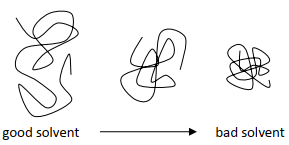
\includegraphics[width=0.50\textwidth]{./Figures/goodbadsolvent.png}
\decoRule
\caption[Effects in polymer chains dimensions due to solvent quality]{Effects in polymer chains dimensions due to solvent quality \cite{Flores2017}}
\label{fig:goodbadsolvent}
\end{figure}

Figure \ref{fig:goodbadsolvent} shows how the quality of a solvent affects the polymer distribution within the solution. Moreover the presence of electrolytes also modify the structure of the polymer threads. In non-ionic solvents, the charges are distributed along the chains and their own repulsion stretches the polymer threads into a more aligned configuration when an electrolyte is added, as detailed in Figure \ref{fig:electrolyteConcentration}.

\begin{figure}[th]
\centering
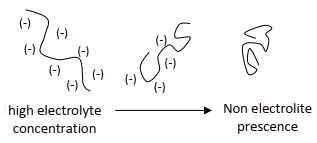
\includegraphics[width=0.50\textwidth]{./Figures/electrolyteConcentration.png}
\decoRule
\caption[Effects of electrolyte in polymer chain dimensions]{Effects of electrolyte in polymer chain dimensions \cite{Flores2017}}
\label{fig:electrolyteConcentration}
\end{figure}

\section{Rheometry}
Rheometry is the measuring technology used to determine rheological data. There are different measuring systems, instruments and analysis methods. Both, liquids and solid  can be investigated using rotational and oscillatory rheometers. Rotational tests are performed to characterize viscous behavior. In order to evaluate viscoelastic behavior, creep tests, relaxation tests and oscillatory tests are performed \cite{Flores2017}.

\subsection{Amplitude Sweep}
An amplitude sweep is a typical test used to characterize the behavior of a polymer
solution or polymer melt. In this basic test a constant angular frequency is applied along with an increasing or decreasing deformation or strain, see Figure \ref{fig:ampSweep} a). The obtained results are the storage and loss moduli, $G'$ and $G''$ respectively, along the values of percentage of strain applied. The amplitude is the maximum of the oscillatory motion. Normally at low frequencies the viscoelastic material presents a linear behavior, this is when the viscoelastic properties are independent of the strain or stress imposed due to the structure of the material stays undisturbed. Nevertheless, as the amplitude is increased at some at some point this linear trend changes suddenly. Once this critical amplitude value is reached the material becomes more elastic or viscous depending on the solution initial state, see Figure \ref{fig:ampSweep} b) \cite{Flores2017}.

\begin{figure}[th]
\centering
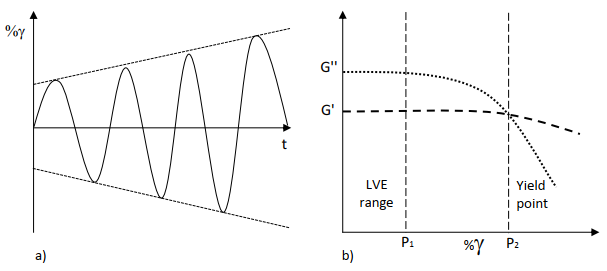
\includegraphics[width=0.75\textwidth]{./Figures/ampSweep.png}
\decoRule
\caption[Amplitude Sweep]{a) Imposed amplitude along time with constant frequency. b) Results for an amplitude sweep \cite{Flores2017}}
\label{fig:ampSweep}
\end{figure}

\subsection{Frequency Sweep}
A frequency sweep, is a common oscillatory test useful to understand the rheological behavior of fluids as it measures the viscoelastic properties. This measurement is considered a viscoelastic spectrum, in general, the shorter the timescale the more elastic the material behaves. These results are related to the molecular structure of the sample. Figure \ref{fig:freqSweep} shows a typical data for a polymer melt where different regions are observed. Frequency sweep measurements also allow the estimation of the molecular weight distribution characteristics such as entanglement density and process-ability \cite{Flores2017}. 

\begin{figure}[th]
\centering
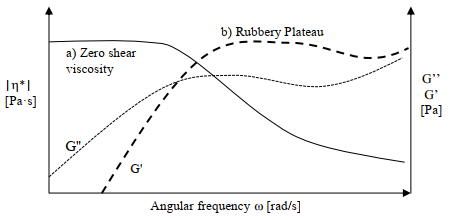
\includegraphics[width=0.75\textwidth]{./Figures/freqSweep.png}
\decoRule
\caption[Frequency Sweep]{Typical results for a frequency sweep. \cite{Flores2017}}
\label{fig:freqSweep}
\end{figure}

\subsection{Flow Curve}
The viscosity is measured as a function of the shear rate in a rotational rheometer with different geometries according to the sample. Normally three types of behaviours can be characterized in flow curve measurements: a) ideal viscous, b) shear thinning and c) shear thickening. Figure \ref{fig:flowCurve} shows three different materials and their response to an imposed shear rate \cite{Flores2017}.

\begin{figure}[th]
\centering
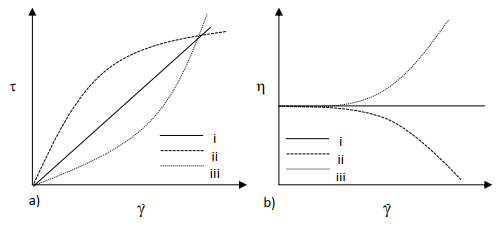
\includegraphics[width=0.75\textwidth]{./Figures/flowCurve.png}
\decoRule
\caption[Flow Curves]{a) Flow curve stress vs stress. b) Flow curve strain vs shear viscosity. Both figures for i Newtonian fluid, ii Shear thinning fluid, iii Shear thickening fluid. \cite{Flores2017}}
\label{fig:flowCurve}
\end{figure}

\section{Preliminary Experiments}

To verify Flores' work \cite{Flores2017}, a series of rheological measurements have been executed. For that purpose, the solutions in Flores work were recreated as follows:

%----------------------------------------------------------------------------------------
%	SECTION 1
%----------------------------------------------------------------------------------------



%-----------------------------------
%	SUBSECTION 1
%-----------------------------------



% Chapter Template

\chapter{Methodology} % Main chapter title

\label{Chapter:Methodology}

%\subsubsection*{\color{mygray}[Chapter under work]}
% process or set of steps that are to take place in order to fulfill the objectives. These steps must mention the experiments to conduct, how they are going to be carried out, the evaluation of the obtained results, the validation of the hypothesis, the answers to the research questions, and the last step must be the written report of the outcomes

The following describes the proposed work to be done to fulfill the objectives stated in this document. The tasks are grouped in several work packages as described bellow:

%----------------------------------------------------------------------------------------
%	SECTION 1
%----------------------------------------------------------------------------------------

\section{Work package 1 : Preliminary Literature Review}
The first step to the thesis development is the study of preliminary literature and related work. The purpose of this work package is the familiarization of the existing techniques such as: far and near field electrospinning, lithography, pyrolysis, carbonization and photopolymerization. On the other hand, some research is to be done in order to recognize if there are any efforts in the design of electrospun-able, photopolymerizable and pyrolysable polymer solutions.

Furthermore, the motive of this work package is to find common parameters that could link the techniques mentioned above for the fabrication of carbon nano-wires from polymer solutions that can be electrospun by NFES, photopolymerized and then pyrolyzed. This work package is to be carried out through the entire thesis development process, as the state-of-the-art may change within that period of time.

\section{Work package 2 : Evaluation of Fabrication Parameters}
As the polymer solution is the principal input to the proposed technique (See Figure \ref{fig:fabricationFlowChart}), it is required to identify and understand the fabrication parameters that have an impact to the quality of the carbon nano-wires. For that reason two tasks are to be executed:

\begin{itemize}
	\item Study and identify the process parameters that influence the fabrication of carbon nano-wires
	\item Study and identify the rheological properties in polymer solutions that affect the electrospinning and pyrolysis techniques
\end{itemize}

\section{Work package 3 : Polymer Solution Design}
Once the process parameters and rheological properties that affect the fabrication of carbon nano-wires are identified, the design process shall take place. This work package is to study polymer solutions that can be electrospun by NFES, photopolymerized and pyrolyzed. The polymer solution design will comprise of two steps:

\begin{itemize}
	\item Prepare and test various polymer solutions with specific distinctions according to the identified solution properties and process parameters.
	\item Perform rheological analyses to determine if the prepared polymer solutions can be employed for the fabrication of carbon nano-wires.
\end{itemize}

\section{Work package 4 : Fabrication of Carbon Nano-wires}
From the rheological analyses, determine and control the polymer solution properties and fabricate carbon nano-wires.
	
This work package intends to involve several manufacturing processes (near field electrospinning, photopolymerization, pyrolization and carbonization) for the fabrication of carbon nano-wires. This task will require the integration of several techniques:

\begin{itemize}
	\item \emph{Electrospinning} - to convert the polymer solution into polymer nano-fibers
	\item \emph{Photopolymerization} - to change the chemical properties of the polymer solution and crosslink its molecules. This is to prevent the polymer to melt during pyrolysis \cite{Basu2018}.
	\item \emph{Pyrolysis} - to transform the polymer nano-fibers into conductive carbon nano-wires.
\end{itemize}

See Figure \ref{fig:fabricationFlowChart}.
	
\section{Work package 5 : Data Collection and Analysis of Results}
The data collection work package comprehends the study of the created carbon nano-wires using the newly design polymer solution. The purpose is characterize the carbon nano-wires and compare them to the carbon nano-structures produced by existing techniques.

\section{Work package 6 : Documentation}
Finally the documentation refers to the Thesis writing tasks. This task is intended to carried out through the entire thesis development process, as every work package above is to be referenced within the thesis document.

%-----------------------------------
%	SUBSECTION 1
%-----------------------------------



% Chapter Template
%\begin{landscape}

\chapter{Work Plan} % Main chapter title

\label{Chapter:WorkPlan}

%\subsubsection*{\color{mygray}[Chapter under work]}
%Once the Methodology has been established, it is important to set up the corresponding activities in an organized and timely manner. This is done using a Workplan Schedule. This provides us a clear idea of the amount of work needed expressed in periods of time.

% move margin to fit table
\leftskip-6em

%%%%%%%%%% 2019 %%%%%%%%%%
% \begin{gantt}{rows}{columns}
\begin{gantt}{11}{12}
\begin{ganttitle}
% \numtitle{from}{step}{to}{width}
\numtitle{2019}{1}{2019}{12}
\end{ganttitle}

\begin{ganttitle}
\numtitle{1}{1}{12}{1}
\end{ganttitle}

% Tasks ...
% \ganttbar{taskName}{start}{duration}
\ganttbar{Preliminary Literature Review}{0}{12}
\ganttbar{Documentation}{0}{12}

\ganttbar{Thesis Kick-off @MTY}{5}{1}
\ganttbar{Evaluation of Fabrication Parameters @MTY}{5}{2}
\ganttbarcon{Polymer Solution Design @CEM}{7}{5}
\ganttbar{Fabrication of Carbon Nano-wires @MTY}{0}{0}
\ganttbar{Data Collection @MTY}{0}{0}
\ganttbar{Analysis of Results @CEM}{0}{0}
\ganttbar{Submit Thesis \& Defend @CEM}{0}{0}

\end{gantt}

%%%%%%%%%% 2020 %%%%%%%%%%
% \begin{gantt}{rows}{columns}
\begin{gantt}{11}{12}
\begin{ganttitle}
% \numtitle{from}{step}{to}{width}
\numtitle{2020}{1}{2020}{12}
\end{ganttitle}

\begin{ganttitle}
\numtitle{1}{1}{12}{1}
\end{ganttitle}

% Tasks ...
% \ganttbar{taskName}{start}{duration}
\ganttbar{Preliminary Literature Review}{0}{12}
\ganttbar{Documentation}{0}{12}

\ganttbar{Thesis Kick-off @MTY}{0}{0}
\ganttbar{Evaluation of Fabrication Parameters @MTY}{0}{0}
\ganttbar{Polymer Solution Design @CEM}{0}{2}
\ganttbarcon{Fabrication of Carbon Nano-wires @MTY}{2}{3}
\ganttbarcon{Data Collection @MTY}{5}{3}
\ganttbarcon{Analysis of Results @CEM}{8}{2}
\ganttbarcon{Submit Thesis \& Defend @CEM}{10}{2}

\end{gantt}

\leftskip-0em
\newpage 

The previous are Gantt diagrams to show the work plan to be executed for the development of the proposed dissertation. The tasks mark with \emph{@CEM} are to be carried out in Tecnológico de Monterrey campus Estado de México; consequently, the tasks mark with \emph{@MTY} are to be performed in Tecnológico de Monterrey campus Monterrey.

%\end{landscape}

%----------------------------------------------------------------------------------------
%	SECTION 1
%----------------------------------------------------------------------------------------



%-----------------------------------
%	SUBSECTION 1
%-----------------------------------




}

%% Chapter 1

\chapter{Chapter Title Here} % Main chapter title

\label{Chapter1} % For referencing the chapter elsewhere, use \ref{Chapter1} 

%----------------------------------------------------------------------------------------

% Define some commands to keep the formatting separated from the content 
\newcommand{\keyword}[1]{\textbf{#1}}
\newcommand{\tabhead}[1]{\textbf{#1}}
\newcommand{\code}[1]{\texttt{#1}}
\newcommand{\file}[1]{\texttt{\bfseries#1}}
\newcommand{\option}[1]{\texttt{\itshape#1}}

%----------------------------------------------------------------------------------------

\section{Welcome and Thank You}
Welcome to this \LaTeX{} Thesis Template, a beautiful and easy to use template for writing a thesis using the \LaTeX{} typesetting system.

If you are writing a thesis (or will be in the future) and its subject is technical or mathematical (though it doesn't have to be), then creating it in \LaTeX{} is highly recommended as a way to make sure you can just get down to the essential writing without having to worry over formatting or wasting time arguing with your word processor.

\LaTeX{} is easily able to professionally typeset documents that run to hundreds or thousands of pages long. With simple mark-up commands, it automatically sets out the table of contents, margins, page headers and footers and keeps the formatting consistent and beautiful. One of its main strengths is the way it can easily typeset mathematics, even \emph{heavy} mathematics. Even if those equations are the most horribly twisted and most difficult mathematical problems that can only be solved on a super-computer, you can at least count on \LaTeX{} to make them look stunning.

%----------------------------------------------------------------------------------------

\section{Learning \LaTeX{}}

\LaTeX{} is not a \textsc{wysiwyg} (What You See is What You Get) program, unlike word processors such as Microsoft Word or Apple's Pages. Instead, a document written for \LaTeX{} is actually a simple, plain text file that contains \emph{no formatting}. You tell \LaTeX{} how you want the formatting in the finished document by writing in simple commands amongst the text, for example, if I want to use \emph{italic text for emphasis}, I write the \verb|\emph{text}| command and put the text I want in italics in between the curly braces. This means that \LaTeX{} is a \enquote{mark-up} language, very much like HTML.

\subsection{A (not so short) Introduction to \LaTeX{}}

If you are new to \LaTeX{}, there is a very good eBook -- freely available online as a PDF file -- called, \enquote{The Not So Short Introduction to \LaTeX{}}. The book's title is typically shortened to just \emph{lshort}. You can download the latest version (as it is occasionally updated) from here:
\url{http://www.ctan.org/tex-archive/info/lshort/english/lshort.pdf}

It is also available in several other languages. Find yours from the list on this page: \url{http://www.ctan.org/tex-archive/info/lshort/}

It is recommended to take a little time out to learn how to use \LaTeX{} by creating several, small `test' documents, or having a close look at several templates on:\\ 
\url{http://www.LaTeXTemplates.com}\\ 
Making the effort now means you're not stuck learning the system when what you \emph{really} need to be doing is writing your thesis.

\subsection{A Short Math Guide for \LaTeX{}}

If you are writing a technical or mathematical thesis, then you may want to read the document by the AMS (American Mathematical Society) called, \enquote{A Short Math Guide for \LaTeX{}}. It can be found online here:
\url{http://www.ams.org/tex/amslatex.html}
under the \enquote{Additional Documentation} section towards the bottom of the page.

\subsection{Common \LaTeX{} Math Symbols}
There are a multitude of mathematical symbols available for \LaTeX{} and it would take a great effort to learn the commands for them all. The most common ones you are likely to use are shown on this page:
\url{http://www.sunilpatel.co.uk/latex-type/latex-math-symbols/}

You can use this page as a reference or crib sheet, the symbols are rendered as large, high quality images so you can quickly find the \LaTeX{} command for the symbol you need.

\subsection{\LaTeX{} on a Mac}
 
The \LaTeX{} distribution is available for many systems including Windows, Linux and Mac OS X. The package for OS X is called MacTeX and it contains all the applications you need -- bundled together and pre-customized -- for a fully working \LaTeX{} environment and work flow.
 
MacTeX includes a custom dedicated \LaTeX{} editor called TeXShop for writing your `\file{.tex}' files and BibDesk: a program to manage your references and create your bibliography section just as easily as managing songs and creating playlists in iTunes.

%----------------------------------------------------------------------------------------

\section{Getting Started with this Template}

If you are familiar with \LaTeX{}, then you should explore the directory structure of the template and then proceed to place your own information into the \emph{THESIS INFORMATION} block of the \file{main.tex} file. You can then modify the rest of this file to your unique specifications based on your degree/university. Section \ref{FillingFile} on page \pageref{FillingFile} will help you do this. Make sure you also read section \ref{ThesisConventions} about thesis conventions to get the most out of this template.

If you are new to \LaTeX{} it is recommended that you carry on reading through the rest of the information in this document.

Before you begin using this template you should ensure that its style complies with the thesis style guidelines imposed by your institution. In most cases this template style and layout will be suitable. If it is not, it may only require a small change to bring the template in line with your institution's recommendations. These modifications will need to be done on the \file{MastersDoctoralThesis.cls} file.

\subsection{About this Template}

This \LaTeX{} Thesis Template is originally based and created around a \LaTeX{} style file created by Steve R.\ Gunn from the University of Southampton (UK), department of Electronics and Computer Science. You can find his original thesis style file at his site, here:
\url{http://www.ecs.soton.ac.uk/~srg/softwaretools/document/templates/}

Steve's \file{ecsthesis.cls} was then taken by Sunil Patel who modified it by creating a skeleton framework and folder structure to place the thesis files in. The resulting template can be found on Sunil's site here:
\url{http://www.sunilpatel.co.uk/thesis-template}

Sunil's template was made available through \url{http://www.LaTeXTemplates.com} where it was modified many times based on user requests and questions. Version 2.0 and onwards of this template represents a major modification to Sunil's template and is, in fact, hardly recognisable. The work to make version 2.0 possible was carried out by \href{mailto:vel@latextemplates.com}{Vel} and Johannes Böttcher.

%----------------------------------------------------------------------------------------

\section{What this Template Includes}

\subsection{Folders}

This template comes as a single zip file that expands out to several files and folders. The folder names are mostly self-explanatory:

\keyword{Appendices} -- this is the folder where you put the appendices. Each appendix should go into its own separate \file{.tex} file. An example and template are included in the directory.

\keyword{Chapters} -- this is the folder where you put the thesis chapters. A thesis usually has about six chapters, though there is no hard rule on this. Each chapter should go in its own separate \file{.tex} file and they can be split as:
\begin{itemize}
\item Chapter 1: Introduction to the thesis topic
\item Chapter 2: Background information and theory
\item Chapter 3: (Laboratory) experimental setup
\item Chapter 4: Details of experiment 1
\item Chapter 5: Details of experiment 2
\item Chapter 6: Discussion of the experimental results
\item Chapter 7: Conclusion and future directions
\end{itemize}
This chapter layout is specialised for the experimental sciences, your discipline may be different.

\keyword{Figures} -- this folder contains all figures for the thesis. These are the final images that will go into the thesis document.

\subsection{Files}

Included are also several files, most of them are plain text and you can see their contents in a text editor. After initial compilation, you will see that more auxiliary files are created by \LaTeX{} or BibTeX and which you don't need to delete or worry about:

\keyword{example.bib} -- this is an important file that contains all the bibliographic information and references that you will be citing in the thesis for use with BibTeX. You can write it manually, but there are reference manager programs available that will create and manage it for you. Bibliographies in \LaTeX{} are a large subject and you may need to read about BibTeX before starting with this. Many modern reference managers will allow you to export your references in BibTeX format which greatly eases the amount of work you have to do.

\keyword{MastersDoctoralThesis.cls} -- this is an important file. It is the class file that tells \LaTeX{} how to format the thesis. 

\keyword{main.pdf} -- this is your beautifully typeset thesis (in the PDF file format) created by \LaTeX{}. It is supplied in the PDF with the template and after you compile the template you should get an identical version.

\keyword{main.tex} -- this is an important file. This is the file that you tell \LaTeX{} to compile to produce your thesis as a PDF file. It contains the framework and constructs that tell \LaTeX{} how to layout the thesis. It is heavily commented so you can read exactly what each line of code does and why it is there. After you put your own information into the \emph{THESIS INFORMATION} block -- you have now started your thesis!

Files that are \emph{not} included, but are created by \LaTeX{} as auxiliary files include:

\keyword{main.aux} -- this is an auxiliary file generated by \LaTeX{}, if it is deleted \LaTeX{} simply regenerates it when you run the main \file{.tex} file.

\keyword{main.bbl} -- this is an auxiliary file generated by BibTeX, if it is deleted, BibTeX simply regenerates it when you run the \file{main.aux} file. Whereas the \file{.bib} file contains all the references you have, this \file{.bbl} file contains the references you have actually cited in the thesis and is used to build the bibliography section of the thesis.

\keyword{main.blg} -- this is an auxiliary file generated by BibTeX, if it is deleted BibTeX simply regenerates it when you run the main \file{.aux} file.

\keyword{main.lof} -- this is an auxiliary file generated by \LaTeX{}, if it is deleted \LaTeX{} simply regenerates it when you run the main \file{.tex} file. It tells \LaTeX{} how to build the \emph{List of Figures} section.

\keyword{main.log} -- this is an auxiliary file generated by \LaTeX{}, if it is deleted \LaTeX{} simply regenerates it when you run the main \file{.tex} file. It contains messages from \LaTeX{}, if you receive errors and warnings from \LaTeX{}, they will be in this \file{.log} file.

\keyword{main.lot} -- this is an auxiliary file generated by \LaTeX{}, if it is deleted \LaTeX{} simply regenerates it when you run the main \file{.tex} file. It tells \LaTeX{} how to build the \emph{List of Tables} section.

\keyword{main.out} -- this is an auxiliary file generated by \LaTeX{}, if it is deleted \LaTeX{} simply regenerates it when you run the main \file{.tex} file.

So from this long list, only the files with the \file{.bib}, \file{.cls} and \file{.tex} extensions are the most important ones. The other auxiliary files can be ignored or deleted as \LaTeX{} and BibTeX will regenerate them.

%----------------------------------------------------------------------------------------

\section{Filling in Your Information in the \file{main.tex} File}\label{FillingFile}

You will need to personalise the thesis template and make it your own by filling in your own information. This is done by editing the \file{main.tex} file in a text editor or your favourite LaTeX environment.

Open the file and scroll down to the third large block titled \emph{THESIS INFORMATION} where you can see the entries for \emph{University Name}, \emph{Department Name}, etc \ldots

Fill out the information about yourself, your group and institution. You can also insert web links, if you do, make sure you use the full URL, including the \code{http://} for this. If you don't want these to be linked, simply remove the \verb|\href{url}{name}| and only leave the name.

When you have done this, save the file and recompile \code{main.tex}. All the information you filled in should now be in the PDF, complete with web links. You can now begin your thesis proper!

%----------------------------------------------------------------------------------------

\section{The \code{main.tex} File Explained}

The \file{main.tex} file contains the structure of the thesis. There are plenty of written comments that explain what pages, sections and formatting the \LaTeX{} code is creating. Each major document element is divided into commented blocks with titles in all capitals to make it obvious what the following bit of code is doing. Initially there seems to be a lot of \LaTeX{} code, but this is all formatting, and it has all been taken care of so you don't have to do it.

Begin by checking that your information on the title page is correct. For the thesis declaration, your institution may insist on something different than the text given. If this is the case, just replace what you see with what is required in the \emph{DECLARATION PAGE} block.

Then comes a page which contains a funny quote. You can put your own, or quote your favourite scientist, author, person, and so on. Make sure to put the name of the person who you took the quote from.

Following this is the abstract page which summarises your work in a condensed way and can almost be used as a standalone document to describe what you have done. The text you write will cause the heading to move up so don't worry about running out of space.

Next come the acknowledgements. On this page, write about all the people who you wish to thank (not forgetting parents, partners and your advisor/supervisor).

The contents pages, list of figures and tables are all taken care of for you and do not need to be manually created or edited. The next set of pages are more likely to be optional and can be deleted since they are for a more technical thesis: insert a list of abbreviations you have used in the thesis, then a list of the physical constants and numbers you refer to and finally, a list of mathematical symbols used in any formulae. Making the effort to fill these tables means the reader has a one-stop place to refer to instead of searching the internet and references to try and find out what you meant by certain abbreviations or symbols.

The list of symbols is split into the Roman and Greek alphabets. Whereas the abbreviations and symbols ought to be listed in alphabetical order (and this is \emph{not} done automatically for you) the list of physical constants should be grouped into similar themes.

The next page contains a one line dedication. Who will you dedicate your thesis to?

Finally, there is the block where the chapters are included. Uncomment the lines (delete the \code{\%} character) as you write the chapters. Each chapter should be written in its own file and put into the \emph{Chapters} folder and named \file{Chapter1}, \file{Chapter2}, etc\ldots Similarly for the appendices, uncomment the lines as you need them. Each appendix should go into its own file and placed in the \emph{Appendices} folder.

After the preamble, chapters and appendices finally comes the bibliography. The bibliography style (called \option{authoryear}) is used for the bibliography and is a fully featured style that will even include links to where the referenced paper can be found online. Do not underestimate how grateful your reader will be to find that a reference to a paper is just a click away. Of course, this relies on you putting the URL information into the BibTeX file in the first place.

%----------------------------------------------------------------------------------------

\section{Thesis Features and Conventions}\label{ThesisConventions}

To get the best out of this template, there are a few conventions that you may want to follow.

One of the most important (and most difficult) things to keep track of in such a long document as a thesis is consistency. Using certain conventions and ways of doing things (such as using a Todo list) makes the job easier. Of course, all of these are optional and you can adopt your own method.

\subsection{Printing Format}

This thesis template is designed for double sided printing (i.e. content on the front and back of pages) as most theses are printed and bound this way. Switching to one sided printing is as simple as uncommenting the \option{oneside} option of the \code{documentclass} command at the top of the \file{main.tex} file. You may then wish to adjust the margins to suit specifications from your institution.

The headers for the pages contain the page number on the outer side (so it is easy to flick through to the page you want) and the chapter name on the inner side.

The text is set to 11 point by default with single line spacing, again, you can tune the text size and spacing should you want or need to using the options at the very start of \file{main.tex}. The spacing can be changed similarly by replacing the \option{singlespacing} with \option{onehalfspacing} or \option{doublespacing}.

\subsection{Using US Letter Paper}

The paper size used in the template is A4, which is the standard size in Europe. If you are using this thesis template elsewhere and particularly in the United States, then you may have to change the A4 paper size to the US Letter size. This can be done in the margins settings section in \file{main.tex}.

Due to the differences in the paper size, the resulting margins may be different to what you like or require (as it is common for institutions to dictate certain margin sizes). If this is the case, then the margin sizes can be tweaked by modifying the values in the same block as where you set the paper size. Now your document should be set up for US Letter paper size with suitable margins.

\subsection{References}

The \code{biblatex} package is used to format the bibliography and inserts references such as this one \parencite{Reference1}. The options used in the \file{main.tex} file mean that the in-text citations of references are formatted with the author(s) listed with the date of the publication. Multiple references are separated by semicolons (e.g. \parencite{Reference2, Reference1}) and references with more than three authors only show the first author with \emph{et al.} indicating there are more authors (e.g. \parencite{Reference3}). This is done automatically for you. To see how you use references, have a look at the \file{Chapter1.tex} source file. Many reference managers allow you to simply drag the reference into the document as you type.

Scientific references should come \emph{before} the punctuation mark if there is one (such as a comma or period). The same goes for footnotes\footnote{Such as this footnote, here down at the bottom of the page.}. You can change this but the most important thing is to keep the convention consistent throughout the thesis. Footnotes themselves should be full, descriptive sentences (beginning with a capital letter and ending with a full stop). The APA6 states: \enquote{Footnote numbers should be superscripted, [...], following any punctuation mark except a dash.} The Chicago manual of style states: \enquote{A note number should be placed at the end of a sentence or clause. The number follows any punctuation mark except the dash, which it precedes. It follows a closing parenthesis.}

The bibliography is typeset with references listed in alphabetical order by the first author's last name. This is similar to the APA referencing style. To see how \LaTeX{} typesets the bibliography, have a look at the very end of this document (or just click on the reference number links in in-text citations).

\subsubsection{A Note on bibtex}

The bibtex backend used in the template by default does not correctly handle unicode character encoding (i.e. "international" characters). You may see a warning about this in the compilation log and, if your references contain unicode characters, they may not show up correctly or at all. The solution to this is to use the biber backend instead of the outdated bibtex backend. This is done by finding this in \file{main.tex}: \option{backend=bibtex} and changing it to \option{backend=biber}. You will then need to delete all auxiliary BibTeX files and navigate to the template directory in your terminal (command prompt). Once there, simply type \code{biber main} and biber will compile your bibliography. You can then compile \file{main.tex} as normal and your bibliography will be updated. An alternative is to set up your LaTeX editor to compile with biber instead of bibtex, see \href{http://tex.stackexchange.com/questions/154751/biblatex-with-biber-configuring-my-editor-to-avoid-undefined-citations/}{here} for how to do this for various editors.

\subsection{Tables}

Tables are an important way of displaying your results, below is an example table which was generated with this code:

{\small
\begin{verbatim}
\begin{table}
\caption{The effects of treatments X and Y on the four groups studied.}
\label{tab:treatments}
\centering
\begin{tabular}{l l l}
\toprule
\tabhead{Groups} & \tabhead{Treatment X} & \tabhead{Treatment Y} \\
\midrule
1 & 0.2 & 0.8\\
2 & 0.17 & 0.7\\
3 & 0.24 & 0.75\\
4 & 0.68 & 0.3\\
\bottomrule\\
\end{tabular}
\end{table}
\end{verbatim}
}

\begin{table}
\caption{The effects of treatments X and Y on the four groups studied.}
\label{tab:treatments}
\centering
\begin{tabular}{l l l}
\toprule
\tabhead{Groups} & \tabhead{Treatment X} & \tabhead{Treatment Y} \\
\midrule
1 & 0.2 & 0.8\\
2 & 0.17 & 0.7\\
3 & 0.24 & 0.75\\
4 & 0.68 & 0.3\\
\bottomrule\\
\end{tabular}
\end{table}

You can reference tables with \verb|\ref{<label>}| where the label is defined within the table environment. See \file{Chapter1.tex} for an example of the label and citation (e.g. Table~\ref{tab:treatments}).

\subsection{Figures}

There will hopefully be many figures in your thesis (that should be placed in the \emph{Figures} folder). The way to insert figures into your thesis is to use a code template like this:
\begin{verbatim}
\begin{figure}
\centering

\includegraphics{Figures/Electron}
\decoRule
\caption[An Electron]{An electron (artist's impression).}
\label{fig:Electron}
\end{figure}
\end{verbatim}
Also look in the source file. Putting this code into the source file produces the picture of the electron that you can see in the figure below.

\begin{figure}[th]
\centering

\includegraphics{Figures/Electron}
\decoRule
\caption[An Electron]{An electron (artist's impression).}
\label{fig:Electron}
\end{figure}

Sometimes figures don't always appear where you write them in the source. The placement depends on how much space there is on the page for the figure. Sometimes there is not enough room to fit a figure directly where it should go (in relation to the text) and so \LaTeX{} puts it at the top of the next page. Positioning figures is the job of \LaTeX{} and so you should only worry about making them look good!

Figures usually should have captions just in case you need to refer to them (such as in Figure~\ref{fig:Electron}). The \verb|\caption| command contains two parts, the first part, inside the square brackets is the title that will appear in the \emph{List of Figures}, and so should be short. The second part in the curly brackets should contain the longer and more descriptive caption text.

The \verb|\decoRule| command is optional and simply puts an aesthetic horizontal line below the image. If you do this for one image, do it for all of them.

\LaTeX{} is capable of using images in pdf, jpg and png format.

\subsection{Typesetting mathematics}

If your thesis is going to contain heavy mathematical content, be sure that \LaTeX{} will make it look beautiful, even though it won't be able to solve the equations for you.

The \enquote{Not So Short Introduction to \LaTeX} (available on \href{http://www.ctan.org/tex-archive/info/lshort/english/lshort.pdf}{CTAN}) should tell you everything you need to know for most cases of typesetting mathematics. If you need more information, a much more thorough mathematical guide is available from the AMS called, \enquote{A Short Math Guide to \LaTeX} and can be downloaded from:
\url{ftp://ftp.ams.org/pub/tex/doc/amsmath/short-math-guide.pdf}

There are many different \LaTeX{} symbols to remember, luckily you can find the most common symbols in \href{http://ctan.org/pkg/comprehensive}{The Comprehensive \LaTeX~Symbol List}.

You can write an equation, which is automatically given an equation number by \LaTeX{} like this:
\begin{verbatim}
\begin{equation}
E = mc^{2}
\label{eqn:Einstein}
\end{equation}
\end{verbatim}

This will produce Einstein's famous energy-matter equivalence equation:
\begin{equation}
E = mc^{2}
\label{eqn:Einstein}
\end{equation}

All equations you write (which are not in the middle of paragraph text) are automatically given equation numbers by \LaTeX{}. If you don't want a particular equation numbered, use the unnumbered form:
\begin{verbatim}
\[ a^{2}=4 \]
\end{verbatim}

%----------------------------------------------------------------------------------------

\section{Sectioning and Subsectioning}

You should break your thesis up into nice, bite-sized sections and subsections. \LaTeX{} automatically builds a table of Contents by looking at all the \verb|\chapter{}|, \verb|\section{}|  and \verb|\subsection{}| commands you write in the source.

The Table of Contents should only list the sections to three (3) levels. A \verb|chapter{}| is level zero (0). A \verb|\section{}| is level one (1) and so a \verb|\subsection{}| is level two (2). In your thesis it is likely that you will even use a \verb|subsubsection{}|, which is level three (3). The depth to which the Table of Contents is formatted is set within \file{MastersDoctoralThesis.cls}. If you need this changed, you can do it in \file{main.tex}.

%----------------------------------------------------------------------------------------

\section{In Closing}

You have reached the end of this mini-guide. You can now rename or overwrite this pdf file and begin writing your own \file{Chapter1.tex} and the rest of your thesis. The easy work of setting up the structure and framework has been taken care of for you. It's now your job to fill it out!

Good luck and have lots of fun!

\begin{flushright}
Guide written by ---\\
Sunil Patel: \href{http://www.sunilpatel.co.uk}{www.sunilpatel.co.uk}\\
Vel: \href{http://www.LaTeXTemplates.com}{LaTeXTemplates.com}
\end{flushright}
 

%----------------------------------------------------------------------------------------
%	BIBLIOGRAPHY
%----------------------------------------------------------------------------------------

\printbibliography[title={References}]

%----------------------------------------------------------------------------------------
%	THESIS CONTENT - APPENDICES
%----------------------------------------------------------------------------------------

\appendix % Cue to tell LaTeX that the following "chapters" are Appendices

% Include the appendices of the thesis as separate files from the Appendices folder
% Uncomment the lines as you write the Appendices

%% Appendix A

\chapter{Frequently Asked Questions} % Main appendix title

\label{AppendixA} % For referencing this appendix elsewhere, use \ref{AppendixA}

\section{How do I change the colors of links?}

The color of links can be changed to your liking using:

{\small\verb!\hypersetup{urlcolor=red}!}, or

{\small\verb!\hypersetup{citecolor=green}!}, or

{\small\verb!\hypersetup{allcolor=blue}!}.

\noindent If you want to completely hide the links, you can use:

{\small\verb!\hypersetup{allcolors=.}!}, or even better: 

{\small\verb!\hypersetup{hidelinks}!}.

\noindent If you want to have obvious links in the PDF but not the printed text, use:

{\small\verb!\hypersetup{colorlinks=false}!}.

%\include{Appendices/AppendixB}
%\include{Appendices/AppendixC}

%----------------------------------------------------------------------------------------

\end{document}  
